\label{sec:druid}
\begin{figure*}[tb]
\centering
\begin{subfigure}[b]{0.33\linewidth}
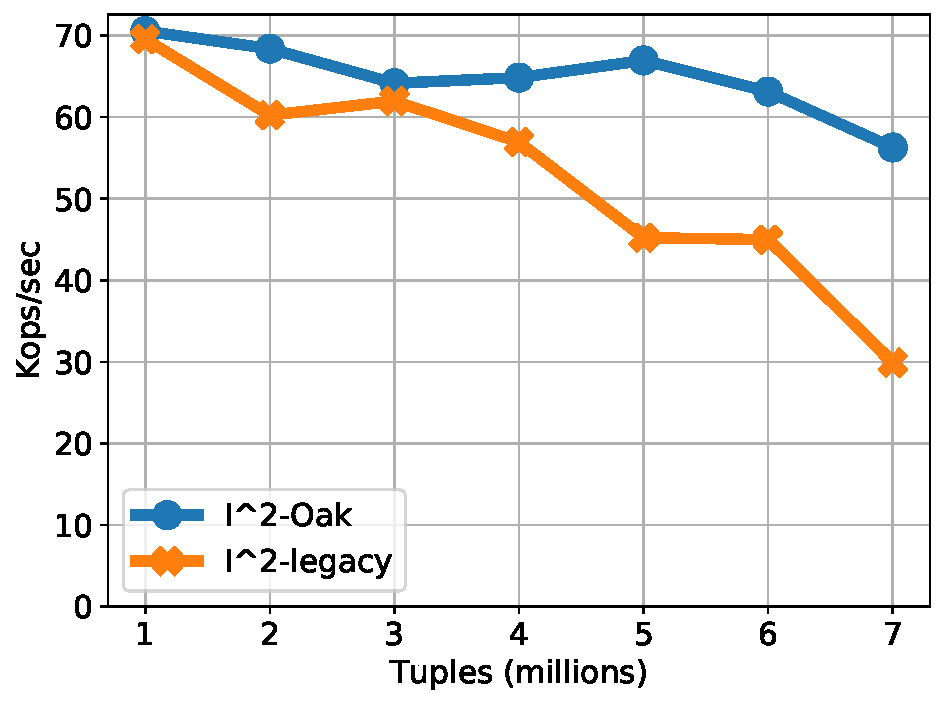
\includegraphics[width=\textwidth]{figs/druid_ingest_30g.pdf}
\vskip -.1in
\caption{Throughput, 30GB RAM, varying dataset}
\label{fig:druid_ingest_32gb_ram}
\end{subfigure}
\begin{subfigure}[b]{0.33\linewidth}
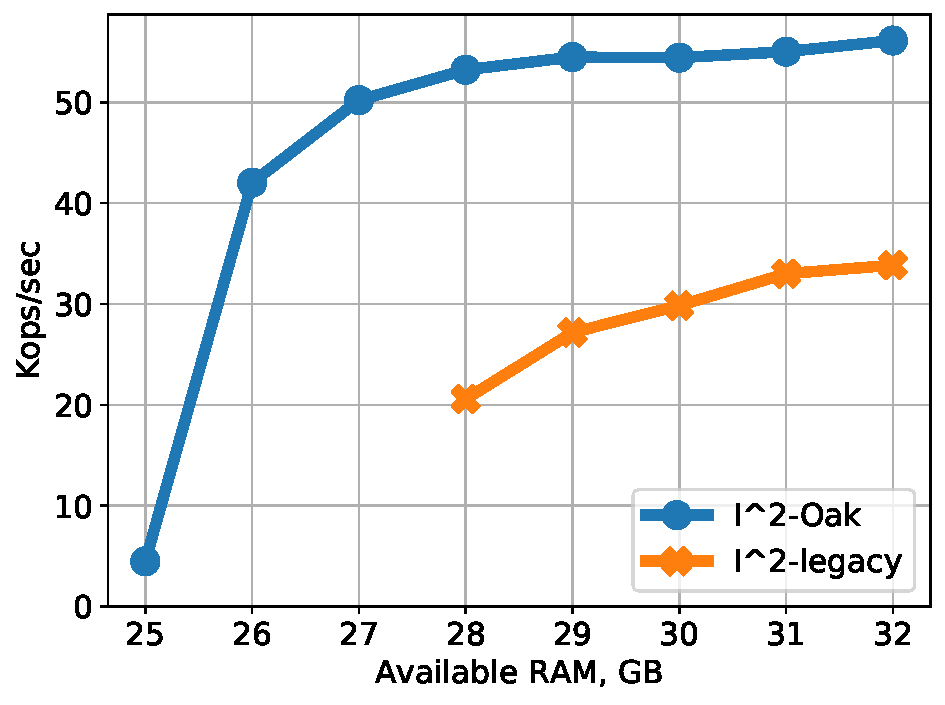
\includegraphics[width=\textwidth]{figs/druid_ingest.pdf}
\vskip -.1in
\caption{Throughput, 7M tuples, varying RAM}
\label{fig:druid_ingest_7m_kv}
\end{subfigure}
\begin{subfigure}[b]{0.33\linewidth}
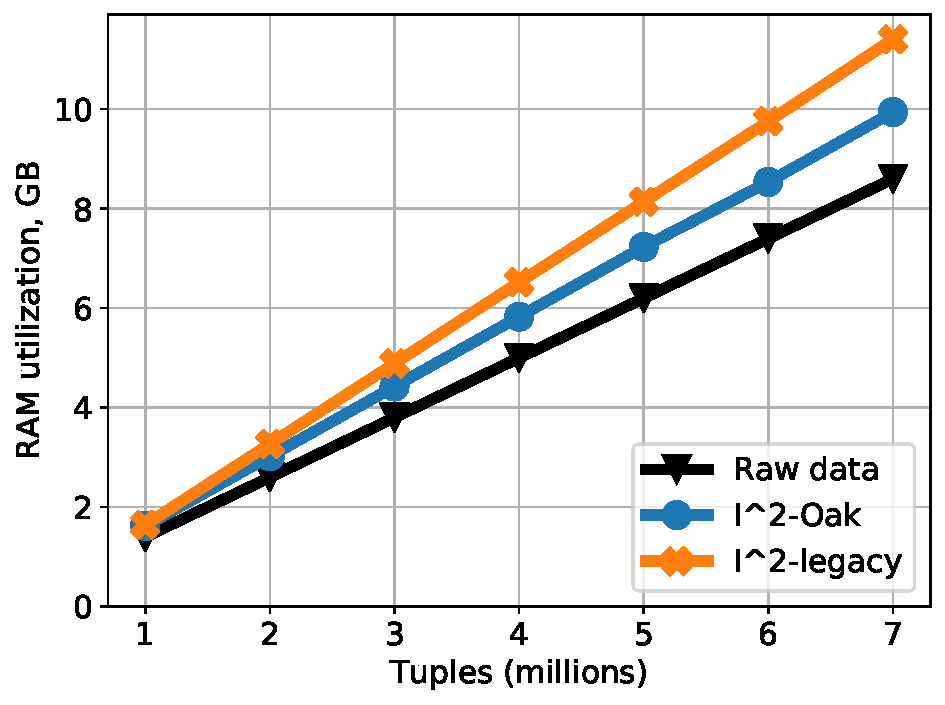
\includegraphics[width=\textwidth]{figs/druid_mem_usage_total.pdf}
\vskip -.1in
\caption{RAM overhead}
\label{fig:druid_mem_usage_total}
\end{subfigure}
\label{fig:druid}
\caption{Single-thread ingestion performance, Druid incremental index: (a,b) throughput, (c) memory efficiency. } 
\end{figure*}

This section presents a case study of \oak's applicability for real-time analytics platforms. 
We build a prototype integration of \oak\ into Apache Druid~\cite{Druid} -- a popular open-source distributed 
analytics database in Java. Our goal is to enable faster ingestion and  improve RAM utilization, which, in turn,  
can lead to I/O reduction. The code, which might be further productized, is under community review~\cite{OakDruidIssue}.

More specifically, we target Druid's \emph{Incremental Index} (\II) component, a  data structure that absorbs new data 
while serving queries in parallel. Data is never removed from an \II. Once an \II\  fills up,  its data gets reorganized and 
persisted, and the \II\ is disposed; the data's further lifecycle is beyond the scope of this discussion. 

\II\/ keys and values are multi-dimensional. In {\em plain\/} \II's, the values are raw data, whereas in {\em rollup\/}
\II's they are materialized aggregate functions. Complex aggregates (e.g., unique count and quantiles) are embodied 
through {\em sketches}~\cite{DruidSketches} -- compact data structures for approximate statistical queries; the rest
are numeric counters. In order to save space, variable-size (e.g., string) dimensions are mapped to numeric codewords, 
through auxiliary dynamic dictionaries. A key maps to a flat array of integers; time is always 
the primary dimension. Keys are typically up to a few hundreds of bytes long. Values are usually up to a few KBs long in 
rollups, and may vary widely in plain indexes. For every incoming data tuple, \II\/ updates its internal KV-map, creating 
a new pair if the tuple's key is absent, or updating in-situ otherwise.

%\paragraph{\oak\/ integration.}  
We re-implement  \II\ by switching the internal map from the JDK ConcurrentSkiplistMap 
to \oak; the auxiliary data structures remain on-heap. 
We implement an adaption layer that controls the internal data layout 
and provides \oak\/ with the appropriate lamdba functions for serialization, deserialization, and in-situ 
compute. The write path exploits \oak's \algvar{putIfAbsentComputeIfPresent()} API for atomic 
update of multiple aggregates within a single lambda. The read path adapts the \II\/ tuple abstraction
to \oak's ZC API. Namely, the new tuple implementation is a lightweight facade to off-heap memory, 
operating atop \oak\/ buffers.

\paragraph{Evaluation.} 
We evaluate the speed and memory utilization of data ingestion with the new solution, \II-\oak,
versus the legacy implementation, \II-legacy. 
The first experiment generates 1M to 7M unique tuples of size 1.25K and feeds them into the index, 
in a single thread. The primary dimension is the current timestamp (in ms), (i.e., the  workload is spatially-local). 
In order to measure ingestion performance in isolation, all the input is generated in advance. 

Figure~\ref{fig:druid_ingest_32gb_ram} depicts the throughput scaling with dataset size, for a fixed RAM budget 
of 30GB. \II-\oak\/ is up to 1.8x faster, e.g., its ingestion speed for 7M tuples (8.6GB 
raw data) is 56K tuples/sec, whereas  \II-legacy's is  30K. Figure~\ref{fig:druid_ingest_7m_kv} 
studies the 7M-tuple dataset under varying memory budget. We see that \II-legacy with 32GB RAM is  more than 25\% slower than
\II-\oak\/ with 26GB RAM, and cannot run with less than 28GB.

Finally, Figure~\ref{fig:druid_mem_usage_total} underscores, \II-\oak's 
memory efficiency. We see that \II-\oak\/ induces at most 15.5\% metadata overhead (including \oak's index and the on-heap 
auxiliary data structures), whereas \II-legacy's space overhead is as high as 32.5\%. 


%Note that \II-\oak's real footprint is much smaller (less than 20GB) because it does not need the 
%pre-generated tuples once they are consumed; \II-legacy references that data from within the index.}



